%%%%%%%%%%%%%%%%%%%%%%%%%%%%%%%%%%%%%%%%%%%%%%%%%%%%%%%%%%%%%%%%%%%%%%
% How to use writeLaTeX: 
%
% You edit the source code here on the left, and the preview on the
% right shows you the result within a few seconds.
%
% Bookmark this page and share the URL with your co-authors. They can
% edit at the same time!
%
% You can upload figures, bibliographies, custom classes and
% styles using the files menu.
%
%%%%%%%%%%%%%%%%%%%%%%%%%%%%%%%%%%%%%%%%%%%%%%%%%%%%%%%%%%%%%%%%%%%%%%

\documentclass[12pt]{article}
\pagenumbering{roman}
\usepackage{sbc-template}
\usepackage{natbib}
\usepackage{graphicx}
\usepackage{graphicx,url}

%\usepackage[brazil]{babel}   
\usepackage[utf8]{inputenc}  

     
\sloppy

\title{Utilizacao de Metricas de Otimizacao para aprimoramento de Rotas}

\author{Marcos Junio da Silva Xavier, Bruna Pereira Passos}


\address{Departamento de Computacao - Centro Federal de Educacao Tecnologica de Minas Gerais \\
  (CEFET-MG)\\
Belo Horizonte -- MG -- Brazil
\email{\{201622040368,201712130080\}@aluno.cefetmg.br}
}
\begin{document} 
\maketitle
\begin{resumo} 
Este artigo apresenta uma forma de otimizar um problema de transporte objetivando traçar a melhor rota de uma empresa. Tal problema pode ser modelado como o problema do Caixeiro Viajante, que possui como características, encontrar uma solução ótima de um determinado roteiro de entregas com menor tempo e menor custo, passando por todas as cidades sem visitar uma mesma cidade duas vezes e retornando à cidade de origem(sede). Para isso, realizou-se a implementação no Python que possui o solver do CPLEX, que é um resolvedor de problemas matemáticos de alto desempenho para programação linear.
Na implementação do código do problema supracitado, variou-se a quantidade de pontos de origens, pontos de destinos, demandas e ofertas, a fim de se realizar uma análise comparativa do tempo de processamento do código.  Ou seja, a análise foi feita em relação ao desempenho, o tempo computacional gasto em cada forma de solução, além disso, verificou-se também a capacidade de se obter a solução ótima.
Obteve-se como conclusão que para problemas de maiores dimensões, o software CPLEX apresentou os melhores índices de desempenho. Já para problemas de pequeno porte a Heurística desenvolvida mostrou-se obter de forma mais rapida uma solucao factivel.

\vspace{\onelineskip}
\noindent
\textbf{Palavras-chaves}: Otimizacao, Modelagem Matematica,
\end{resumo}
\begin{abstract}This article presents a way of optimizing a transportation problem in order to map the best route of a company. Such a problem can be modeled as the Traveling Salesman problem, which has as its features, finding an optimal solution of a given route with less time and less cost, passing all cities without visiting the same city twice and returning to the city. source. For this, the implementation was performed in Python with CPLEX solver, which is a high performance mathematical problem solver for linear programming, generating precise and logical decisions, thus allowing to optimize decisions, reduce costs and increase profitability. In implementing the code, the number of source points, destination points, demands and offers was varied in order to perform a comparative analysis of code processing time. That is, the analysis was performed in relation to the performance, the computational time spent on each form of solution, and also the ability to obtain the optimal solution. It was concluded that for larger problems, the CPLEX software presented the best performance indexes, but with variations in time, which may not be acceptable for a software. For small problems, the developed Heuristic has always shown a feasible solution faster.

\vspace{\onelineskip}
\noindent
\textbf{Key-words}: Optmization, Mathematical Modeling
\end{abstract}
     

\section{Introducao}

Este artigo apresenta uma forma de otimizar um problema para obter melhor rota de carros para entregas por cidades , obtido com dados informados de uma empresa de transporte de valores de abrangência mundial, com uma de suas franquias localizadas no Prado,Belo Horizonte.Tal problema pode ser modelado como o problema do Caixeiro Viajante,que consiste em encontrar uma solução ótima para um determinado roteiro de entregas na rota de maneira eficiente ,ou seja, menor tempo e menor custo, passando por todas as cidades sem visitar uma mesma cidade duas vezes e retornando a cidade de origem(sede).Foi tomada como decisão de implementação utilizar a linguagem de Programação Python, pois possui a biblioteca solver do CPLEX,um resolvedor de problemas matemáticas de alto desempenho para programação linear ,gerando decisões precisas e lógicas,permitindo assim otimizar decisões para melhor eficiência,reduzir custos e aumentar a lucratividade.
Dados alguns problemas devido a sua grande devido a sua enorme dificuldade de uma solução e a representatividade em larga escala de situações no cotidiano,Problemas de Otimização Combinatória tem exigido que programas mais eficientes sejam criados .
Assim, para a solução do problema abordado, iremos atribuir valores a um conjunto de variáveis de decisão,uma vez que será determinado a função objetivo a qual se deseja otimizar,neste caso, a intenção será minimizar a função objetivo, devendo atender a um conjunto de restrições.
Uma forma não eficiente de uma solução para esse problema, permeia a  elaborar de um algoritmo que de forma gulosa, ou seja, não preocupando com a melhor resposta, encontre uma solução factível,uma solução que atenda a função objetivo e ao conjunto de restrições.Porém, essa técnica se torna impraticável, pois se aumentarmos o número de variáveis, pode-se demorar um tempo inadmissível para aguardar a resposta , seja em horas, ou dias.Por isso, faz-se necessários o uso de técnicas em conjunto com a computação e a otimização para resolver esses problemas de combinação.



\section{Trabalhos Relacionados}

A gestão do transporte nas organizações implica a tomada de decisões sobre como movimentar materiais e produtos acabados entre diferentes pontos de uma determinada rede de negócios. Na abordagem tradicional, a gestão do transporte é discutida principalmente em questões operacionais de seus fluxos (Mason, Ribera, Farris, & Kirk, 2003; Neuschel & Russell, 1998; Ng, Ferrin, & Pearson, 1997), medido em sua performance operacional e custos (McCann, 2001; Meixell & Norbis, 2008). O artigo “COMPARAÇÃO DE DESEMPENHO E USABILIDADE ENTRE OS SOFTWARES COMERCIAIS DE OTIMIZAÇÃO E O MÉTODO DUAL PARA O PROBLEMA CLÁSSICO DO TRANSPORTE” destaca que gerando diferentes instâncias aleatórias, variando quantidade de pontos de origens, pontos de destinos, demandas e ofertas, pode-se analisar o desempenho, avaliar o tempo computacional gasto em cada forma de solução, em relação à eficácia e também analisar a relação de usabilidade, avaliar-se a interface com o usuário, a dificuldade de aprendizagem e a linguagem de programação necessária. Silva (2012) desenvolveu sua pesquisa
utilizando um modelo exato, executado através do solver GLPK (Gnu Linear
Programming Toolkit), para encontrar a solução ótima. Bezerra (2013) desenvolveu seu
trabalho utilizando o Algoritmo Genético (AG) para buscar uma aproximação da
solução ótima.


\section{Definição Formal e Algoritmo Heurístico}
Problemas como o Caixeiro Viajante pode ser classificado como NP-Completo, ou seja, problemas de difícil solução.
Dado um grafo G = (N, E) onde N = {1, ..., n} é o conjunto de vértices e E = {1, ...,m} é o conjunto de arestas de G. O custo Cij representa o custo associado a aresta que liga os vértices i e j. O problema consist,e em determinar o menor ciclo hamiltoniano do
grafo G, sendo que o tamanho do ciclo é dado pelo somatório dos custos das arestas que o compõem .
Transportando para aprimoramento de rotas, se usarmos os termos “Cidades” ao invés de vértices e “Custo” relativo à distância entre dois pontos no lugar de aresta o problema poderia ser reescrito como: calcular o percurso com menor custo de um conjunto de visitas partindo de um  ponto, percorrendo todos os outros, uma única vez e, ao final, voltando ao ponto inicial.
Grafos criados pelo problema do caixeiro viajante são em sua maioria determinado como simétrico: Não direcionado, uma vez que possibilita que seja criada uma rota para ir e voltar contando que seja a mesma distancia.Porem na pratica ,sabe-se que existem ruas ou avenidas de mão única, o qual não permite a volta por essa mesma rota, assim, devemos adotar um grafo hibrido, tendo em sua maioria arestas de retorno com tamanho igual a aresta de ida,



Dado um conjunto  C=\{c_1\;,...,\;c_n\}}  de n cidade c_i  e uma matriz de distancias p_ij = p(c_i,c_j) (i,j ) \in 1,...n

Para a modelagem do problema proposto utilizamos a seguinte função :
Para a funcao objetivo, temos:\newline

\sum_{i=1}^{M}\sum_ {j=1}^{N} CijXij\newline

Para o conjunto de restrições :\newline

\sum_{i=1}^{N} Xij, $ i \mid i\neq $j =1 \forall  i \newline

\sum_{j=1}^{N} Xij, $ i \mid i\neq $j =1 \forall  j \newline

 {u_i > = q_i \forall i} 
 
 Onde ,\newline
  c_{ij}     =
  Custo de ir da cidade i a cidade j (distância).
 \newline
 
Com os grafos cada cidade é identificada com um nó e as rotas que ligam cada par de nós são como arcos. A cada uma destas linhas estarão associadas as distâncias ou os custos correspondentes. Desde que seja possível ir diretamente de uma cidade para qualquer outra, o gráfico diz-se completo. A distância do ciclo é o somatório das distâncias das linhas presentes no mesmo. (Bank, 1996)
O problema pode ser representado por um grafo tal que os custos sejam associados a cada uma das arestas. No caso real em que o grafo completo com  cidades é encontrar o melhor circuito entre os  possíveis. 
 
\subsection{Heuristica}
Desenvolvemos um programa ,utilizando a Linguagem C,apartir dos conhecimentos obtidos nas disciplinas ofertadas pelo DECOM- Departamento de Cmputacao do CEFET, tais como , Algoritmos e Estrutura de Dados,com o intuito de criar uma heuristica para gerar uma instancia gulosa  e uma solucao completamente aleatoria para o problema.

Os resultados da heuristica serao apresentados no proximo capitulo.
\section{Resultados}
Apos a simulação dos dados criados para testar o programa desenvolvido, o CPLEX encontrou a solução em um tempo extremamente ótimo,para esse caso.

Reduced MIP has 268 binaries, 0 generals, 0 SOSs, and 234 indicators.

Presolve time = 0.00 sec. (0.78 ticks)

Probing time = 0.01 sec. (1.30 ticks)

Clique table members: 687.

MIP emphasis: balance optimality and feasibility.

MIP search method: dynamic search.

Parallel mode: deterministic, using up to 4 threads.

Root relaxation solution time = 0.00 sec. (0.39 ticks)


Clique cuts applied:  29

Cover cuts applied:  559

Implied bound cuts applied:  251

Flow cuts applied:  1

Mixed integer rounding cuts applied:  2

Zero-half cuts applied:  44

Gomory fractional cuts applied:  2

Root node processing (before b&amp;c):

  Real time             =    0.22 sec. (71.55 ticks)
  
Parallel b&amp;c, 4 threads:

  Real time             =  119.79 sec. (57043.83 ticks)
  
  Sync time (average)   =   11.56 sec.
  
  Wait time (average)   =    0.05 sec.
  
                          ------------
Total (root+branch&amp;cut) =  120.00 sec. (57115.37 ticks)



As variáveis que devem entrar na função objetivo ,determinada pelo CPLEX ao qual minimiza a função objetivo e retorna  o mínimo da função sao \:


x_{010} = 1 

x_{40} = 1

x_{017} = 1

x_{160} = 1

x_{616} = 1

x_{130} = 1

x_{145} = 1

x_{150} = 1

x_{011} = 1

x_{127} = 1

x_{913} = 1

x_{1715} = 1

x_{50} = 1

x_{012} = 1

x_{70} = 1

x_{118} = 1

x_{06} = 1

x_{09} = 1

x_{84} = 1

x_{03} = 1

x_{314} = 1

x_{12} = 1

x_{1001} = 1

x_{20} = 1




u_1 = 14.000

u_2 = 15.000

u_3 = 5.000

u_4 = 14.000

u_5 = 15.000

u_6 = 4.000

u_7 = 15.000

u_8 = 10.000

u_9 = 5.000

u_10 = 8.000

u_11 = 7.000

u_12 = 9.000

u_13 = 14.000

u_14 = 7.000

u_15 = 15.000

u_16 = 12.000

u_17 = 8.000\newline\end{multicols}
Onde u ea variavel de demanda.


Dado esse resultado, a funcao objetivo fica :

Min (F_x) =  97172  \*  x_{010} + 67784  \*  x_{40} + 225014  \*  x_{017} +162268  \*  x_{16 0} + 119738  \*  x_{6 16}+141397  \*  x_{13 0} +197744  \*  x_{14 5}+239216  \*  x_{15 0}+116474  \*  x_{0 11} + 89282  \*  x_{12 7}+Cij  \*  x_{9 13} +19008  \*  x_{17 15} +232159  \*  x_{15 0}+176081  \*  x_{0 12 }+ 108259  \*  x_{7 0}+ 107319  \*  x_{11 8}+51265  \*  x_{0 6}+103292  \*  x_{0 9} +157712  \*  x_{8 4}+ 193014  \*  x_{0 3 } +209551  \*  x_{13 14 }+ 28939  \*  x_{1 2}+77102  \*  x_{10 1}+ 180079  \*  x_{2 0}}\newline
\newpage
Foi possivel obter pelo CPLEX  figuras contendo o grafo do caminho percorrido, iniciando da sede,Belo Horizonte,como podemos ver na imagem abaixo :
\begin{center}
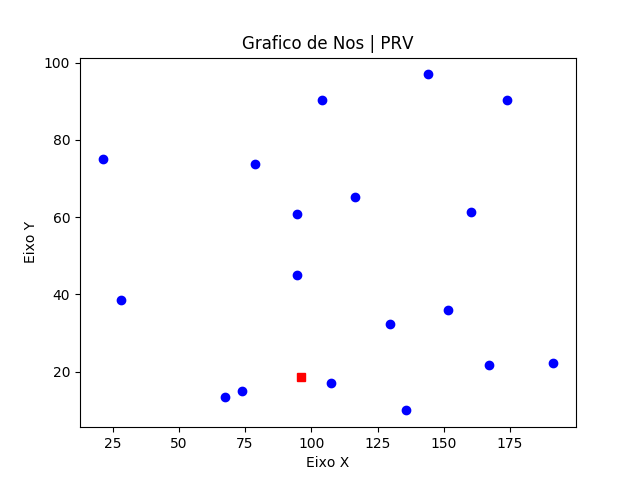
\includegraphics[scale=0.9]{Figure_11}} 
\caption{Figura 1}
\end{center}Na Figura 1 , podemos visualizar a dispersao dos pontos,representados pelas cidades.A Cidade de origem(sede)foi desenhada pelo no em vermelho, e em seguida as demais seguintes cidades foram desenhadas com nos coloridos em azul. 

\begin{center}    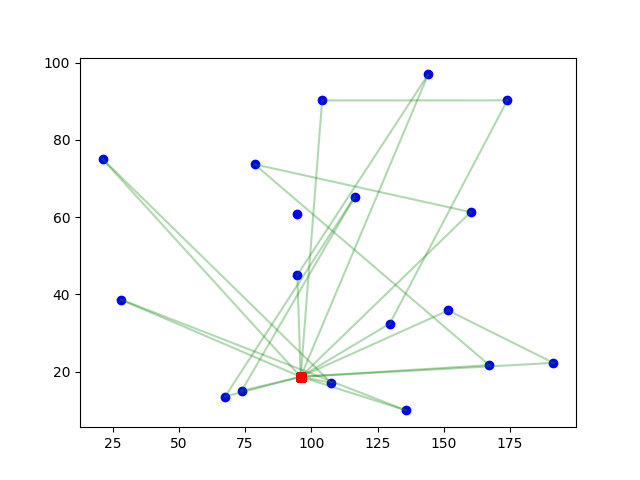
\includegraphics[scale=0.9]{Figure_12}
    \caption{Figura 2}\end{center}
Na figura 2,podemos visualizar que apos o CPLEX a procura do menor caminho, construiu umaa rota que atende a restricao do problema. 
\begin{center}
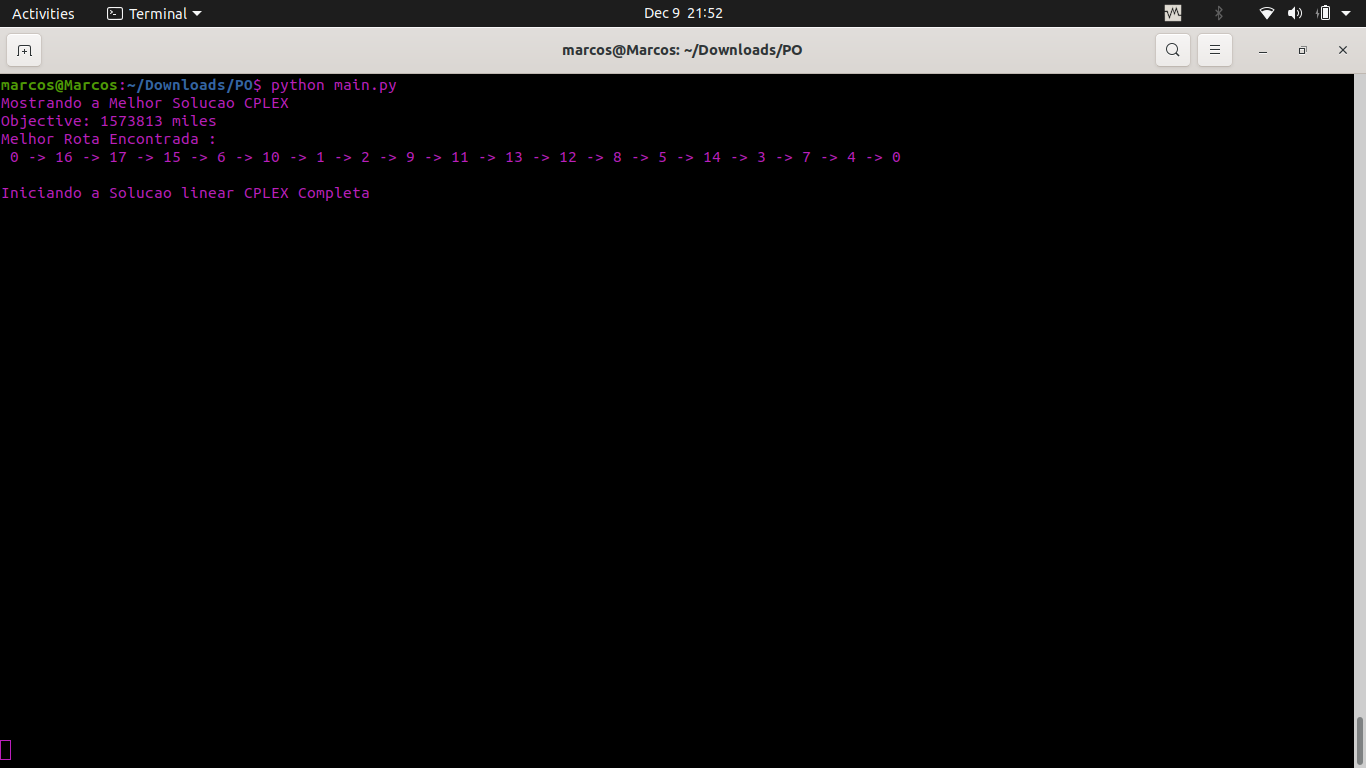
\includegraphics[scale=0.35]{cplex_completo.png}} 
\caption{Figura 3}
\end{center}

Na Figura 3, podemos visualizar a resposta do CPLEX para o melhor caminho para a entrada proposta, mostrando como 0 a cidade de origem(sede) e percorrendo todas as 17 cidades seguintes e depois retornando a cidade de origem.
1573813 km foi considerado como distancia minima para percorrer as 17 cidades.

\begin{center}
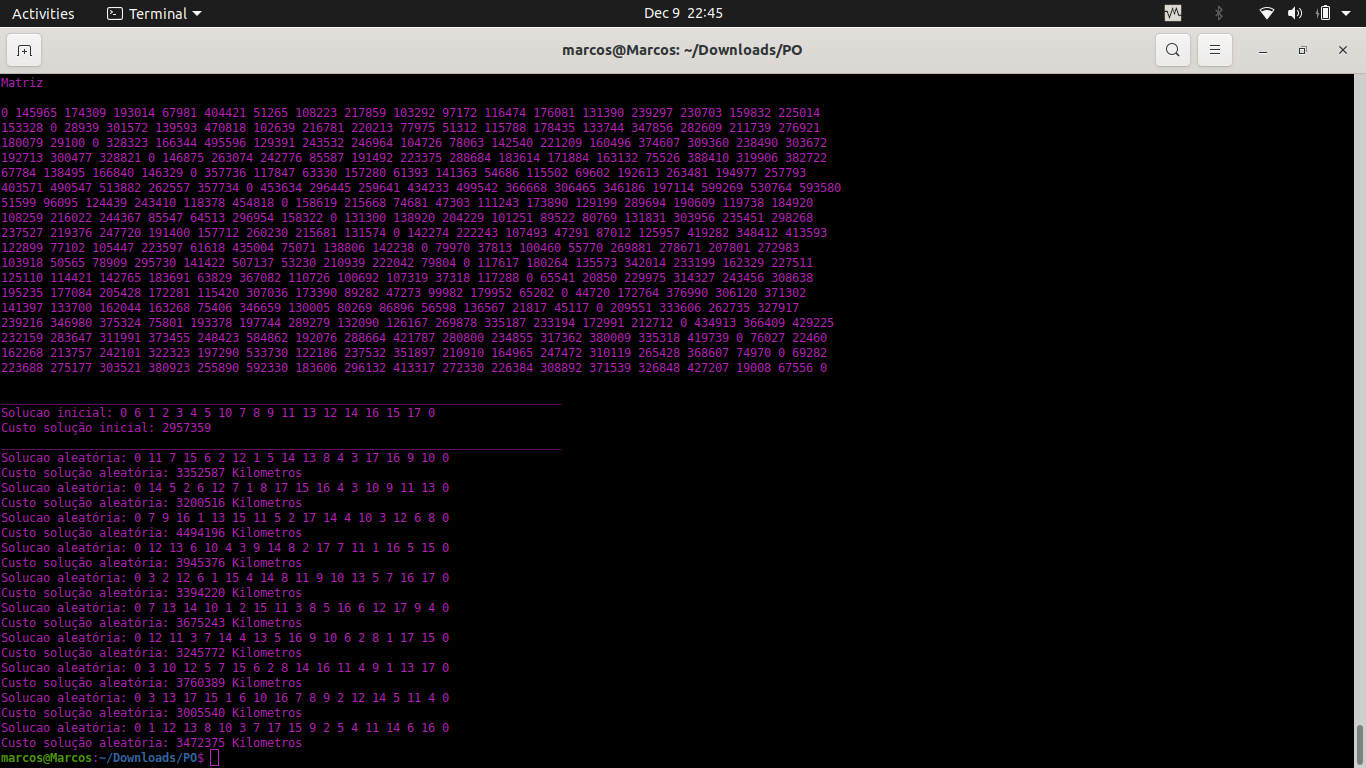
\includegraphics[scale=0.35]{solucao_aleatoria.png}} 
\caption{Figura 4}
\end{center}
Na Figura 4, mostra o resultado da heuristica implementada para encontrar alguma solucao aleatoria para o problema.Pode se perceber que inumeras solucoes sao aceitas, porem,a distancia percorrida foi considerada bastante significativa , pois houve casos em que foi possivel percorrer as 17 cidades rodando um total de 4494196 km.
\section{Conclusão}
O Objetivo deste trabalho e de auxiliar empresas que utilizam rotas para determinar caminhos de visitas para que sejam feitas entregas, visitas,etc com o intuito de minimizar o tempo de viagem , assim ,possibilitando maximizar lucros . 
Para testar as instancias, foi criado uma heurística gulosa e comparada com o CPLEX foi possível perceber que existem varias rotas que podem ser utilizadas, porem, a rota sugerida pelo CPLEX contem a rota de menor tempo de viagem.
\subsection{Problemas encontrados}
Algumas dificuldades foram detectadas durante a implantação deste trabalho, sendo elas:\newline
• Criar o roteiro com o tempo entre dois pontos sendo assimétrico. Então, um conjunto de instancias mais controlada foi escolhida com tempo simétricos.
.
 
\newpage
\section{Referencias}

KHOROV, E.; KIRYANOV, A.; LYAKHOV, A.; BIANCHI, G. A Tutorial on IEEE 802.11ax High Efficiency WLANs.

\newline GRIBKOVSKAIA, I.; LAPORTE, G.; SHYSHOU, A. The single vehicle routing problem with deliveries and selective pickups. Computers & Operations Research. [S. l.], v. 35, p. 2908-2924, 2008.

\newline LIAO, X.; TING, C. An Evolutionary Approach for the Selective Pickup and Delivery Problem. Evolutionary Computation. [S. l.], 2010.

\newline BRUCK, B. P.; SANTOS, A. G.; ARROYO, J. E. C. Hybrid metaheuristic for the single vehicle routing problem with deliveries and selective pickups. IEEE World Congress on Computational Intelligence, p. 1-8, 2012a.

\newline COELHO, I. M. et al. A hybrid heuristic based on General Variable Neighborhood Search for the Single Vehicle Routing Problem with Deliveries and Selective Pickups. Electronic Notes in Discrete Mathematics. [S. l.], v. 39, p. 99-106, 2012.

\newline WANG, X.; DESSOUKY, M.; ORDÓÑEZ, F. A Pickup and Delivery Problem for Ridesharing Considering Congestion. Transportation Letters. [S. l.], v. 8, p. 259-269, 2016.

\newline CERVIERI, Alexandre; PY, Mónica – Algoritmo para a resolução do problema do caixeiro viajante [Em Linha]. Porto Alegre: Instituto de Informática - UFRGS, 2000. [Consult. 5 Dezembro. 2019]. 

\newline MANSO, S. J., Ribera, M. P., Farris, J. A., & Kirk, R. G. (2003). Integrating the warehousing and transportation functions of the supply chain. Transportation Research Part E: Logistics and Transportation Review].

\newline FRANTE, J. Alexandre. Comparação de desenvolvimento e usabilidade entre os softwares comerciais de otimização e o método dual para o problema clássico do transporte. Acesso em <https://www.marinha.mil.br/spolm/sites/www.marinha.mil.br.spolm/files/115229.pdf>

\newline SIQUEIRA, Paulo Henrique; STEINER, Maria Teresinha Arns; SCHEER, Sérgio – A new approach to solve the traveling salesman problem [Em Linha]. Amsterdam: ScienceDirect - Neurocomputing: A new approach to solve the traveling salesman problem, 2006. [Consult. 09 Dezembro. 2019].

\newline BEZERRA, T. L. A.; Algoritmo Genético Aplicado ao Problema de Roteamento de
Veículos nas Entregas Realizadas por uma Empresa de Laticínios: Estudo de Caso.
53 f. Monografia (Graduação em Ciência e Tecnologia) – Universidade Federal
Rural do Semi-Árido, Angicos. 2013. 

\newline Silva, G. L. S.; Roteamento de veículos nas entregas realizadas por empresa de
laticínios - estudo de caso. 52 f. Monografia (Graduação em Ciência e Tecnologia) –
Universidade Federal Rural do Semi-Árido, Angicos. 2012.

\end{document}
